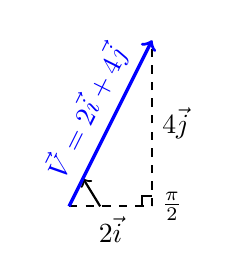
\begin{tikzpicture}[scale=1.5]

\draw [thick, dashed] (0,0) -- ++(2em, 0)
	node [pos=0.5, below] {$2\vec{i}$};
\draw [thick, dashed] (2em, 0) -- ++(0, 4em)
	node [pos=0.5, right] {$4\vec{j}$};

\draw [thick] (1.75em, 0em) |- (2em, 0.25em);
\node at (2em, 0) [right] {$\frac{\pi}{2}$};

\draw [thick, ->] (0.75em, 0em) -- (63:0.75em);

\draw [very thick, blue, ->] (0,0) -- ++(2em, 4em)
	node [pos=0.5, above, sloped]
	{$\vec{V} = 2\vec{i} + 4\vec{j}$};
\end{tikzpicture}
